% !TeX spellcheck = cs_CZ
%=============== Kapitola: Antény: Teoretický základ ===============================================
\setchaptertoc
\chapter{Antény: Teoretický základ}\label{chap:ra_antennatheory}


  \section{Teoretický základ}
    Když jsme se na počátku našeho výkladu zabývali šířením vln, nezajímali jsme se o to, jak vlny 
    vznikly. Proces vzniku vlnění v prostoru (proces vyzařování) bude vyšetřováno v této kapitole. 
    
    Z fyziky je známo, že zdrojem elektromagnetických vln je střídavý (vysokofrekvenční) proud. 
    Úlohu o vyzařování můžeme tedy formulovat tak, že známe proud tekoucí v prostoru (na vysílací 
    anténě) a chceme zjistit, jaké intenzity polí vytvoří tento proud kdekoli jinde v prostoru. 
    Matematicky jde o \textbf{řešení nehomogenní soustavy Maxwellových rovnic:}
    \begin{align}\label{RA:eq_ant01}
      \rot{H} &= \vec{J} + j\omega\varepsilon\vec{H} \\
      \rot{E} &= -j\omega\mu\vec{H}
    \end{align}
    v níž proudová hustota \(\vec{J}\) je známá a intenzity \(\vec{E}\) a \(\vec{H}\) se hledají 
    \cite[s.~33]{Hanus2002}. 
    
    \subsection{Impedance lineárních antén}
      Lineární anténa je \emph{jednobran} a poměr fázorů vstupního napětí a vstupního proudu 
      definuje  tzv. \textbf{vstupní impedanci antény}. Vstupní impedance je veličina stejně 
      důležitá jako funkce záření, protože rozhoduje o přizpůsobení antény k napájecímu vedení. 
      Vstupní impedance je obecně komplexní: má reálnou část (\emph{vstupní odpor}) a imaginární 
      část (\emph{vstupní reaktanci}). Obě složky bezprostředně souvisí s činností antény. Anténa 
      vyzařuje jistý činný výkon, a tudíž nejméně stejný činný výkon musí také odebírat ze zdroje. 
      Z hlediska uživatele se musí jevit na svorkách antény takový reálný odpor, který by odebíral 
      tentýž výkon. Ve skutečnosti má anténa ztráty (část přivedeného činného výkonu se mění v 
      teplo), takže odebíraný výkon bude o něco větší a odpor na svorkách také. Kromě toho anténa 
      během každé periody si vyměňuje energii s elektromagnetickým polem ve svém blízkém 
      okolí a to se projeví existencí jisté reaktance na vstupu. Této úvaze odpovídá náhradní obvod 
      antény nakreslený na obr. \ref{RA:fig_001} \cite[s.~44]{Hanus2002}.

      \begin{figure}[ht!]   %\ref{RA:fig_001}
        \centering
        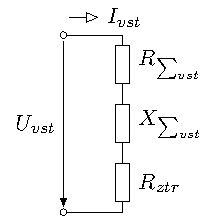
\includegraphics[width=0.5\linewidth]{RA001.pdf}
        \caption{Náhradní obvod antény}
        \label{RA:fig_001}
      \end{figure}
      
      Odpor \(R_{\sum_{vst}}\) je tzv. \textbf{odpor záření antény} vztažený ke vstupnímu proudu. 
      Místo odpor záření se užívají také názvy \emph{vyzařovací odpor} nebo \emph{zářivý odpor}. 
      Odpor  \(R_{ztr}\) je \textbf{ztrátový odpor antény}. V součinu se čtvercem efektivní hodnoty 
      vstupního proudu tyto odpory určují \textbf{vyzařovaný a ztrátový výkon antény}:
      \begin{itemize}[noitemsep]
        \item \emph{vyzařovaný výkon:} \(P_{\sum} = I^2_{vst_{ef}}\cdot R_{\sum_{vst}}\)
        \item \emph{ztrátový výkon:}   \(P_{ztr} = I^2_{ztr_{ef}}\cdot R_{ztr}\)
      \end{itemize}
      Protože na anténě je obvykle stojaté vlnění, je proud v každém místě jiný. Vyzařovaný výkon 
      je však jeden. Podle prvního z uvedených vztahů přísluší tedy každému proudu, a tedy i 
      každému místu na anténě, jiná hodnota odporu záření. Nebo naopak, každá hodnota odporu záření 
      je \emph{vztažena} k určitému proudu (místu) na anténě. Nejčastěji se odpor záření vztahuje 
      buď k proudu vstupnímu (\(I_{vst}\)) nebo k proudu v kmitně (\(I_{max}\)). Vyzařovaný výkon 
      je tedy alternativně
      \begin{equation}\label{RA:eq_ant02}
        P_{\sum} = I^2_{vst_{ef}}\cdot R_{\sum_{vst}} = I^2_{max_{ef}}\cdot R_{\sum_{m}}
      \end{equation} 
      \(R_{\sum_{m}}\) je \emph{odpor záření vztažený ke kmitně proudu}. Vztah (\ref{RA:eq_ant02}) 
      umožňuje přepočítat odpor záření z jednoho místa do druhého, známe-li funkci \emph{proudové 
      distribuce}. 
      
      
     
  \section{Parametry antén}
    Elektrické vlastnosti antén různých typů se charakterizují stručnými číselnými údaji, které 
    nazýváme parametry. Jejich znalost je důležitá při navrhování rádiových soustav 
    \cite[s.~46]{Hanus2002}. 

     % In many situations, a good match is defined arbitrarily as having SWR<1.5. 
     V mnoha aplikacích se dosažené impedanční přizpůsobení považuje dobré je-li \(\text{VSWR}<1,5\)
     \begin{align}
       \text{VSWR} &= \frac{1+\abs{\Gamma}}{1-\abs{\Gamma}} \qquad \Rightarrow \qquad
                     \abs{\Gamma} = \frac{\text{VSWR}-1}{\text{SWR}+1}, \\
       \shortintertext{a odražený výkon lze jednoduše získat jako mocninu amplitudy koeficientu 
         odrazu} 
       R_L &= -10\log\abs{\Gamma}^2 = -20\log\abs{\Gamma} \qquad\unit{\decibel} \\
       \shortintertext{and the transmitted power to the load, relative to the incident wave power, 
         is}
       T_L &= -10\log(1 - \abs{\Gamma}^2) \qquad\unit{\decibel}
     \end{align}
     
     
    \begin{table}[ht!]
      \centering
      \begin{tabular}{c|ccc}
        \rowcolor[HTML]{000000} 
        \multicolumn{1}{c}{\cellcolor[HTML]{000000}
          {\color[HTML]{FFFFFF} \textbf{VSWR}}}      & 
          {\color[HTML]{FFFFFF} \textbf{\(\abs{\Gamma}\)}} & 
        \multicolumn{2}{c}{\cellcolor[HTML]{000000}
          {\color[HTML]{FFFFFF} \textbf{Odražený výkon}}}          \\ 
        \rowcolor[HTML]{000000}{\color[HTML]{FFFFFF} }           &
                               {\color[HTML]{FFFFFF} \(\abs{s_{11}}\)}  & 
                               {\color[HTML]{FFFFFF} (\%)}       & 
                               {\color[HTML]{FFFFFF} (dB)}           \\
         1.0 & 0.000 &  0.0 & \(\infty\)  \\
         1.5 & 0.200 &  4.0 & 14.0  \\
         2.0 & 0.333 & 11.1 & 9.55  \\
         2.5 & 0.429 & 18.4 & 7.36  \\
         3.0 & 0.500 & 25.0 & 6.00  \\
         3.5 & 0.556 & 30.9 & 5.10  \\
         4.0 & 0.600 & 36.0 & 4.44  \\
         5.0 & 0.667 & 44.0 & 3.52  \\
         6.0 & 0.714 & 51.0 & 2.92  \\
         7.0 & 0.750 & 56.3 & 2.50  \\
         8.0 & 0.778 & 60.5 & 2.18  \\
         9.0 & 0.800 & 64.0 & 1.94  \\
        10.0 & 0.818 & 66.9 & 1.74  \\
        15.0 & 0.875 & 76.6 & 1.16  \\
        20.0 & 0.905 & 81.9 & 0.87  \\
        50.0 & 0.961 & 92.3 & 0.35  \\ \cline{1-4}
        \hline
      \end{tabular}
      \caption{Demonstrace vzájemného vztahu mezi poměrem stojatých vln \texttt{VSWR}, amplitudy 
               koeficientu odrazu \(\Gamma\) a velikostí odraženého výkonu\protect\footnotemark[3] 
               vyjádřeného v procentech a decibelech. Kredit: \AntTheoVSWR}
      \label{fig_RA:VSWRGammaTable}
    \end{table}

 \footnotetext[3]{Return loss}

%---------------------------------------------------------------------------------------------------